\section{Introduction}

Bitcoin showed that a peer-to-peer network can stop double spending without a trusted third party \cite{nakamoto}. Its unit, however, is too volatile to price goods or write contracts in \cite{yermack}. Every attempt since to give a cryptocurrency a stable unit trusts somebody: a custodian who holds the reference asset (e-gold, PAX Gold, Tether Gold), the publishers of a price feed (BitShares, Synthetix, Ampleforth), or a second token whose value is meant to absorb shocks (Terra, Basis, Iron Finance). Doing it in a fully decentralized way is still described as an open problem \cite{klagesmundt,caldarelli}. The custodians can fail or be closed, as e-gold was in 2008 \cite{egold-doj}; the feeds can be bribed or pushed, as Mango Markets' was \cite{mango}; and the second-token designs collapsed in runs \cite{terra}.

Zen takes a different route for one particular kind of stable unit: a unit of metal. It has six coins.

\begin{itemize}
\item Three \textbf{physical coins} of fixed weight: the gold \textbf{Ren} (4\,g), the silver \textbf{Ten} (3\,g) and the copper \textbf{Sen} (2\,g). They are ordinary metal, held privately, and worth what their metal is worth.
\item Three \textbf{electronic coins} on three independent public chains: \textbf{Golden Yen}, \textbf{Silver Ken} and \textbf{Bronze Jen}. The goal is $1~\YEN = 1~\REN$, $1~\KEN = 1~\TEN$ and $1~\JEN = 1~\SEN$.
\end{itemize}

Nobody holds metal for the electronic coins, and nobody reports a metal price to the chains. Each chain reads what its physical coin is worth from its own payments. Shops that price in coins (``this bread costs 6 Sen'') pay exact sixths of a coin; everybody else pays arbitrary amounts. Comparing the two tells the network how many of its base units one physical coin buys. The network then sets the weight of its electronic coin, $S$ base units, to that value. The off-chain fact, what a copper coin buys, still enters through people: Zen is an \emph{endogenous} oracle, not ``no oracle''. Fake payments cannot be ruled out without an authority \cite{douceur}, so the design does not try to forbid them. It prices them: each gram counts once, old money counts more than new, receivers post bonds, the reading moves at most 2.9\% a day, and once the three chains trade with each other an attacker must also beat the exchange.

The rest of Zen exists to make that measurement possible at scale and cheap enough for small payments:

\begin{itemize}
\item \textbf{Proof of Minting} (Section~\ref{sec:pom}): ordinary people, including phones, earn the right to prove groups of payments with zero-knowledge proofs by hashing a memory-hard puzzle. Their proofs build each block as a tree, so capacity grows with the number of minters, and they share the fees.
\item \textbf{Mining} (Section~\ref{sec:mining}): miners seal each minted block with SHA-256 over Bitcoin's exact 80-byte header, through ordinary Stratum pools, and win new coins on a curve set by each metal's metallic ratio. Fork choice counts both minting and sealing work.
\item \textbf{Purity} (Section~\ref{sec:purity}): each payment chooses its fee rate, its ``fineness'', and the average purity resizes the chain.
\item \textbf{The coin weight} (Section~\ref{sec:peg}): the self-reading peg and its layered defences.
\item \textbf{A self-correcting system} (Section~\ref{sec:selfcorrect}): why three linked currencies, each tied to a physical coin, can detect an attack, name the chain under attack and pull it back.
\item \textbf{Channels, factories and Zen Net} (Sections~\ref{sec:channels}--\ref{sec:zennet}): payments streamed off-chain across the three metals, and a paid network layer that uses them.
\end{itemize}

\paragraph{Contributions.} This paper (i) describes a complete design for metal-denominated electronic money with no custodian and no price feed; (ii) introduces Proof of Minting, a collaborative block-building scheme in which phones prove payments and share fees by work; (iii) specifies a peg read inside consensus from coin-priced payments, with a set of defences and their measured cost to an attacker; and (iv) reports prototype measurements, devnet tests and simulations for each of them, together with the problems that remain open (Section~\ref{sec:open}).

\paragraph{What Zen does not claim.} Zen measures value in metal. It does not stabilize the price of goods: metal standards gave long-run price stability alongside multi-decade deflations \cite{bordo,eichengreen}. It has no central bank or balance sheet, and every historical commodity scheme that actively stabilized prices had one \cite{bis2018,ussher}. Its claim is narrower: to give everybody a common, manipulation-resistant gram reference without a central party, so that metal becomes usable as a unit of account again.

%=====================================================================
\section{The system at a glance}\label{sec:overview}

\begin{figure}[tbp]
\centering
\begin{tikzpicture}[node distance=6mm and 6mm]
  % physical coins
  \node[box,fill=yen!12,draw=yen,minimum width=3.6cm] (ren) {\textbf{Ren}\\[-1pt]{\scriptsize 4\,g gold coin}};
  \node[box,fill=ken!10,draw=ken,minimum width=3.6cm,right=1.2cm of ren] (ten) {\textbf{Ten}\\[-1pt]{\scriptsize 3\,g silver coin}};
  \node[box,fill=jen!10,draw=jen,minimum width=3.6cm,right=1.2cm of ten] (sen) {\textbf{Sen}\\[-1pt]{\scriptsize 2\,g copper coin}};
  % chains
  \node[box,draw=yen,line width=1.1pt,minimum width=3.6cm,minimum height=1.25cm,below=1.3cm of ren] (yen) {\textbf{Golden Yen}\\[-1pt]{\scriptsize 15-min blocks \textperiodcentered{} limited supply}};
  \node[box,draw=ken,line width=1.1pt,minimum width=3.6cm,minimum height=1.25cm,below=1.3cm of ten] (ken) {\textbf{Silver Ken}\\[-1pt]{\scriptsize 5-min blocks}};
  \node[box,draw=jen,line width=1.1pt,minimum width=3.6cm,minimum height=1.25cm,below=1.3cm of sen] (jen) {\textbf{Bronze Jen}\\[-1pt]{\scriptsize 2.5-min blocks \textperiodcentered{} launches first}};
  \foreach \a/\b/\c in {ren/yen/yen,ten/ken/ken,sen/jen/jen}{
    \draw[arr,dashed,color=\c] (\a) -- node[lbl,right,fill=white,inner sep=1pt] {1 = 1, read\\from payments} (\b);
  }
  % work roles
  \node[box,fill=wash,below=1.0cm of ken,minimum width=12cm] (work) {\textbf{Minters} (phones, PCs): blows, leaves \enspace\textbar\enspace \textbf{Builder} (server, GPU): stamp \enspace\textbar\enspace \textbf{Miners} (SHA-256): seal};
  \foreach \c in {yen,ken,jen}{ \draw[arr] (work.north -| \c) -- (\c.south); }
  % upper layers
  \node[box,fill=bluewash,above=1.0cm of ten,minimum width=12cm] (l2) {\textbf{L2} channels and factories: melt, stream, cast \quad\textbar\quad \textbf{Exchange} between Yen, Ken and Jen};
  \node[box,fill=copperwash,above=4mm of l2,minimum width=12cm] (l3) {\textbf{L3} Zen Net: paid routing, storage and computing, priced in Sen};
  % cross check
  \draw[arr,{Stealth[length=2mm]}-{Stealth[length=2mm]},color=ink2] (yen.east) -- node[lbl,above] {stamps} (ken.west);
  \draw[arr,{Stealth[length=2mm]}-{Stealth[length=2mm]},color=ink2] (ken.east) -- node[lbl,above] {stamps} (jen.west);
\end{tikzpicture}
\caption{Zen's architecture. Three physical coins and three electronic chains; each chain reads its coin's value from its own payments. Minters and miners build every block; channels, the exchange and Zen Net sit on top. The chains verify each other's block proofs (stamps), but none depends on another for validity.}
\label{fig:arch}
\end{figure}

Figure~\ref{fig:arch} shows the parts and Table~\ref{tab:coins} the six coins. The physical coins are the reference and the store of value; the electronic coins are the medium of payment. The three chains are independent: each has its own work, its own block size and its own coin weight, and nothing in one chain's validity rules reads another chain's data \st{Decided}. They do follow each other's headers and check each other's block proofs (164 bytes, about 1\,ms each), so a payment on one chain can be verified on another without a bridge.

\begin{table}[htbp]
\centering\small
\begin{tabularx}{\textwidth}{l l l l Y}
\toprule
\textbf{Physical coin} & \textbf{Metal} & \textbf{Electronic coin} & \textbf{Chain role} & \textbf{Typical use}\\
\midrule
\textcolor{yen}{\textbf{Ren}} & 4\,g gold & Golden Yen (\YEN) & store of value & savings, large settlements, contracts\\
\textcolor{ken}{\textbf{Ten}} & 3\,g silver & Silver Ken (\KEN) & confirmation & salaries, mid-size payments, trade\\
\textcolor{jen}{\textbf{Sen}} & 2\,g copper & Bronze Jen (\JEN) & testing ground, launches first & everyday purchases, small change, streams\\
\bottomrule
\end{tabularx}
\caption{The six coins. The aim is $1~\YEN=1~\REN$, $1~\KEN=1~\TEN$ and $1~\JEN=1~\SEN$.}
\label{tab:coins}
\end{table}

\paragraph{Roles.} A \emph{user} sends and receives payments from a phone wallet. A \emph{minter} hashes the memory-hard blow puzzle and proves groups of payments; a phone can do this. A \emph{builder}, in practice a mining pool, turns the minters' leaves into a block and its stamp on a server with a GPU. A \emph{miner} seals blocks with SHA-256 hardware. A \emph{full node} keeps the state and serves it to minters. A \emph{stream node} runs channels on one or more metals and earns routing and exchange fees. Roles are switched on in one app \st{Decided in principle}.

\paragraph{Launch order.} Jen launches first. Ken starts when Jen's raw block reward first falls below one base unit (Jen block 729,328, about 3.5 years after Jen starts), and Yen when Ken's does (Ken block 21,138, about 73 days after Ken starts) \st{Decided}. Jen is therefore the proving ground for every rule; changes later pass to Ken and then to Yen with rising thresholds (Section~\ref{sec:upgrades}).

%=====================================================================
\section{Chain parameters and issuance}\label{sec:issuance}

Each metal is a separate chain with its own constants (Table~\ref{tab:params}). Three of them come from the \emph{metallic means}, the positive roots of $x^2 - m x - 1 = 0$ for the metallic order $m$:
\begin{equation}
r = \frac{m + \sqrt{m^2+4}}{2}, \qquad a = \frac{\ln 2}{\ln r}.
\end{equation}
Gold takes the golden ratio ($m=1$, $r=1.618$), silver the silver ratio ($m=2$, $r=2.414$) and bronze the bronze ratio ($m=3$, $r=3.303$). The ratio sets each chain's reward exponent $a$ and the spread of its random reward factor.

\begin{table}[htbp]
\centering\small
\begin{tabularx}{\textwidth}{Y r r r l}
\toprule
\textbf{Constant} & \textcolor{yen}{\textbf{Golden Yen}} & \textcolor{ken}{\textbf{Silver Ken}} & \textcolor{jen}{\textbf{Bronze Jen}} & \textbf{Status}\\
\midrule
Metallic order $m$ / ratio $r$ & 1 / 1.6180 & 2 / 2.4142 & 3 / 3.3028 & Decided\\
Reward exponent $a=\ln 2/\ln r$ & 1.440 & 0.786 & 0.580 & Decided\\
Block time & 15 min & 5 min & 2.5 min & Decided\\
Blocks per day & 96 & 288 & 576 & Decided\\
Data ceiling per block & 4 MB & 3 MB & 2 MB & Decided\\
Standard fee (purity target) & 0.1\% & 0.4\% & 1\% & Decided\\
Fee limits per payment & 0.01--2.5\% & 0.01--4.5\% & 0.01--6\% & Decided\\
Initial raw reward & 2,520 & 2,520 & 2,520 & Decided\\
Long-run supply & limited, $\approx$7,255 & grows $\approx N^{0.21}$ & grows $\approx N^{0.42}$ & Open (curve)\\
Smallest unit & $10^{-12}$ (pico) & $10^{-12}$ & $10^{-12}$ & Decided\\
Upgrade activation threshold & 90\% & 75\% & 60\% & Decided\\
Minter share of fees & 75\% & 75\% & 75\% & Open\\
\bottomrule
\end{tabularx}
\caption{Chain parameters (specification section 2).}
\label{tab:params}
\end{table}

\subsection{The reward curve}
The raw reward of block $N$ falls as a power of $N$:
\begin{equation}
\mathrm{Raw}(N) = 2520 \cdot N^{-a}.
\end{equation}
Because $a>1$ for gold, Yen's total supply converges, to about 7,255 coins; for silver and bronze $a<1$, so Ken and Jen grow forever, but ever more slowly, roughly as $N^{0.21}$ and $N^{0.42}$ (Figure~\ref{fig:supply}, Table~\ref{tab:supply}). Gold is scarce and final; copper keeps pace with an economy that keeps needing small change.

\begin{figure}[tbp]
\centering
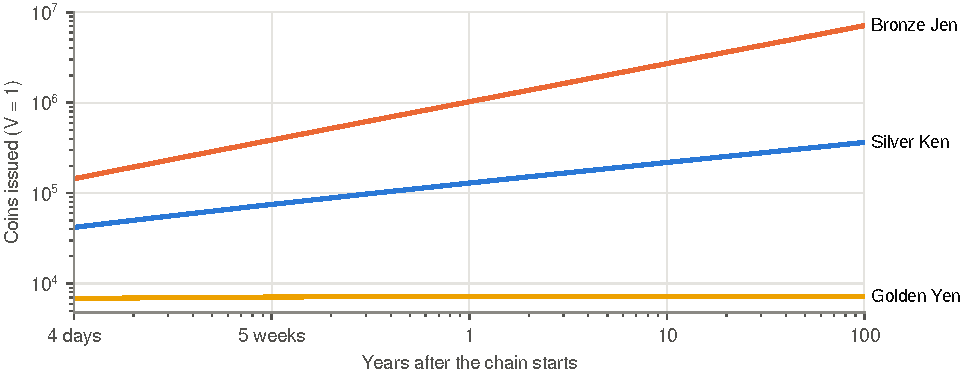
\includegraphics[width=\textwidth]{figs/supply.pdf}
\caption{Coins issued on each chain with the random factor $V=1$ in every block (computed from $\mathrm{Raw}(N)$; log scales). Yen approaches a limit of about 7,255 coins; Ken and Jen keep growing more slowly.}
\label{fig:supply}
\end{figure}

\begin{table}[htbp]
\centering\small
\begin{tabular}{l r r r}
\toprule
\textbf{Supply after} & \textbf{1 year} & \textbf{10 years} & \textbf{100 years}\\
\midrule
\textcolor{yen}{Golden Yen} & 7,198 & 7,234 & 7,247 (limit $\approx$7,255)\\
\textcolor{ken}{Silver Ken} & 129,000 & 218,000 & 362,000\\
\textcolor{jen}{Bronze Jen} & 1,026,000 & 2,706,000 & 7,121,000\\
\bottomrule
\end{tabular}
\caption{Supply with $V=1$ at every block (specification 5.5). The random factor raises the totals by its arithmetic mean, 1.12, 1.47 and 2.04 respectively.}
\label{tab:supply}
\end{table}

\subsection{A random factor that nobody can steer}
Each block's reward is multiplied by a random factor drawn from the \emph{next} block's seal, so no miner can know or influence its own draw \st{Decided}:
\begin{equation}
u = \frac{\mathrm{SHA256}(\mathrm{seal}_{N+1}\,\|\,\text{``reward''})}{2^{256}},\quad Z=\Phi^{-1}(u),\quad V = r^{Z},\quad \mathrm{Reward}(N) = \mathrm{Raw}(N)\cdot V .
\end{equation}
$V$ has a geometric mean (and median) of exactly 1, so a typical block follows the raw curve. All nodes compute it in integers: fixed constants for $\ln r$ and $a$, a fixed-point exponential, and a shared 65,536-entry table for $\Phi^{-1}$ and $r^Z$. There is no floating point in consensus.

\paragraph{The metallic split.} Once $V$ is known, the miner keeps the raw part of the new coins and the block's minters share the windfall above it, scaled by $1/r$ \st{Decided}:
\begin{equation}
\mathrm{Miner}(N) = \begin{cases}\mathrm{Raw}(N)\cdot V & V\le 1\\ \mathrm{Raw}(N)\cdot V^{1/r} & V>1\end{cases}\qquad \mathrm{Minters}(N) = \mathrm{Reward}(N)-\mathrm{Miner}(N).
\end{equation}
The miner's median income stays exactly $\mathrm{Raw}(N)$ and only windfalls are shared, so miners' income is steadier. Because the spread of $V$ grows with $r$, the minters' share grows from gold to bronze (Figure~\ref{fig:split}): on Jen, the everyday chain, minters receive more than half of the new coins on average.

\begin{figure}[htbp]
\centering
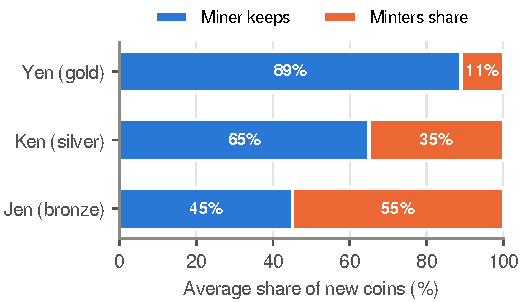
\includegraphics[width=0.62\textwidth]{figs/split.pdf}
\caption{Average split of new coins between the sealing miner and the block's minters (specification 5.4.1). In the top 1\% of Jen blocks $V$ reaches 16.1 and the miner keeps 2.3.}
\label{fig:split}
\end{figure}

%=====================================================================
\section{Accounts and payments}\label{sec:accounts}

Each chain keeps balances in a Merkle tree of accounts; each leaf is the hash of the account's address, balance and nonce, where the address is the hash of the public key, and its root is carried in every block header \st{Decided in principle}. The benchmark tree has depth 32, about 4.3 billion accounts. Every payment is public; privacy lives in the channel layer (Section~\ref{sec:channels}).

\paragraph{Payment format.} Inside a minted block a payment is about 13 bytes: a 4-byte sender index, a 4-byte receiver index, and the amount and fee as variable-length integers in base units (measured: 1,632 bytes for 128 payments). The nonce is implied by the sender's account and the signature is checked inside the proof, so neither is stored. In the pool, with its signature, a payment is about 100--140 bytes \st{TBD byte layout}.

\paragraph{Validity.} A payment is valid when its Schnorr signature on the EcGFp5 curve (prime order $n$, 319 bits; BabyJubjub EdDSA in the Go prototype) signs the Poseidon hash of the chain id, sender, receiver, amount, fee and nonce, with $s < n$; its nonce equals the sender's current nonce; the balance covers amount plus fee; its fee rate $\text{fee}/(\text{amount}+\text{fee})$ is inside the chain's limits; and the amount is at least the smallest payment (Section~\ref{sec:w}) \st{Decided}.

\paragraph{Purity: the payer chooses speed.} Each payment carries its \emph{fineness}, its fee rate expressed like the purity of metal: on Jen, from 940 (a 6\% fee) through the standard 990 (1\%) to 9999 (0.01\%). Minters take the highest fee first, counted in base units: 100~\JEN{} at 1\% (a fee of 1~\JEN) goes before 1~\JEN{} at 6\% (0.06~\JEN). The fineness only has to be inside the limits, so payers choose speed by the fee they pay \st{Decided, revised October 2026}. Under the earlier rule, which ranked by fee rate, on a busy Jen-0.6 devnet payments at 940 confirmed in a median of 15\,s, at 990 in 25\,s and at 9999 in 68\,s; the 9999 payments drained when traffic was quiet (Figure~\ref{fig:purity}). Sending 1~\JEN{} costs its purity in coins: 0.0638~\JEN{} at 940, 0.0101 at 990 and 0.0001 at 9999.

\begin{figure}[htbp]
\centering
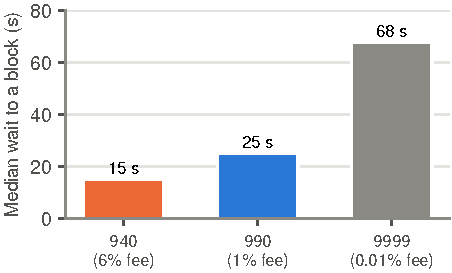
\includegraphics[width=0.55\textwidth]{figs/purity.pdf}
\caption{Fineness and speed on a busy Jen-0.6 devnet, when minters still ranked by fee rate: median time from sending to inclusion in a block (devnet).}
\label{fig:purity}
\end{figure}

\paragraph{New accounts.} A wallet is a key pair made offline; nothing is registered. An account appears in the tree the first time its address receives coins (a payment, a minting share or a mining reward). That first payment carries the 32-byte address once, about 45 bytes in the block; afterwards the account is a 4-byte index. The leaf then lives in the state, not in later blocks, until the account is closed. New accounts need no special spam rule: they compete for block space by fee like any payment, and the first amount must reach the smallest payment \st{Proposed}.

\paragraph{Closing an account.} A payment can close its sender's account with a signed flag: the balance must end at zero and the leaf is emptied, freeing the slot. A new account starts at nonce $\text{height}\times 2^{20}$, above any nonce an earlier account with the same key could have used, so its old signatures can never be replayed \st{Proposed, in the benchmark circuit}.

\paragraph{One address on all three chains.} The same key gives the same address on Yen, Ken and Jen, and a wallet shows it as one account with three balances. Each chain still keeps its own leaf for that address in its own tree, since no chain's rules read another chain's data, so a stall on one chain never freezes the others. Every signed message starts with the chain id, so a payment signed for one chain cannot be replayed on another even when the nonces match. In an exchange, ``to my Ken address'' is simply the trader's address, and a chain can check a payment on another chain against that chain's 196-byte stamp \st{Proposed, in the benchmark circuit}.

\paragraph{Two signatures, optional.} For shops and face-to-face payments, a payment request can ask for the receiver's signature too, and say who pays the fee and at what purity. Nobody can then push payments onto another account, and a wrong address cannot receive without agreeing. Ordinary sends, payroll and donations stay single-signature \st{Proposed}.
